\documentclass[journal]{IEEEtran} % use the `journal` option for ITherm conference style
\IEEEoverridecommandlockouts
\usepackage{graphicx} % Required for inserting images
\usepackage{amsmath,amssymb,amsfonts}
\usepackage{algorithmic}
\usepackage{csquotes}
\usepackage{textcomp}
\usepackage{xcolor}
\usepackage[spanish]{babel}
\usepackage{enumitem}
\usepackage[
backend=biber,
style=ieee,
sorting=none
]{biblatex}
\addbibresource{references.bib}

\renewcommand{\IEEEkeywordsname}{Palabras clave}
\def\BibTeX{{\rm B\kern-.05em{\sc i\kern-.025em b}\kern-.08em
    T\kern-.1667em\lower.7ex\hbox{E}\kern-.125emX}}
\graphicspath{ {Images/} }

\title{Diseño y arquitectura de un sistema inteligente para el monitoreo de colmenas apícolas}
\author{%%%% author names
    \IEEEauthorblockN{Ing. Carlos Humberto Montaño Alcala}
    , \IEEEauthorblockN{M.C. Rafael Armando Galaz Bustamante*}
    , \IEEEauthorblockN{Dra. María Trinidad Serna Encinas}
    , \IEEEauthorblockN{Dr. Omar Hernández González}
    , \IEEEauthorblockN{Dra. Rosalía Del Carmen Gutiérrez Urquídez}
    \vspace{1cm}
    \vfill
    \IEEEauthorblockN{Tecnológico Nacional de México/Instituto Tecnológico de Hermosillo, División de Estudios de Posgrado e Investigación. Av. Tecnológico 115, Col. Sahuaro, CP. 83170,Hermosillo, Sonora, México.
    \vfill
    }
    \IEEEauthorblockN{Correos: m16330894@hermosillo.tecnm.mx, rafael.galazb@hermosillo.tecnm.mx, maria.sernae@hermosillo.tecnm.mx , omar.hernandezg@hermosillo.tecnm.mx , rosalia.gutierrezu@hermosillo.tecnm.mx 
    }
}
\date{September 2024}

\begin{document}

\maketitle

\begin{abstract}
     La apicultura es una actividad esencial para la producción de miel y otros productos derivados de las abejas, así como para la polinización de plantas. En México, la apicultura juega un papel significativo, siendo el noveno productor de miel a nivel mundial. El estado de Sonora, aunque contribuye con solo el 7\% de la producción nacional de miel, destaca por la utilización de sus colmenas, principalmente para la polinización de cultivos. Para asegurar la salud y producción eficiente de las colmenas, es necesario contar con un monitoreo constante, que tradicionalmente se realiza de manera manual, con un apicultor visitando la colmena cada 8 a 15 días en búsqueda de anomalías y enfermedades. Con el aumento de colmenas, este proceso manual puede volverse ineficiente y tardado, añadiendo requerimientos de logística y el riesgo de no monitorear las colmenas en el tiempo recomendado. Esta investigación propone el desarrollo de un sistema de monitoreo de colmenas apícolas utilizando técnicas de Internet de las Cosas (IoT), con el fin de mejorar la eficiencia y efectividad del monitoreo. El sistema integrará sensores para medir variables como temperatura, humedad, peso y audio, y empleará un algoritmo de reconocimiento de patrones para identificar eventos de interés que puedan requerir la atención del apicultor. Se desarrollará una aplicación móvil para la visualización de los datos recopilados y los resultados del procesamiento. Este sistema tiene como objetivo proporcionar a los apicultores información en tiempo real sobre el estado de sus colmenas, mejorando así la toma de decisiones y optimizando el manejo de las colmenas.
     
\end{abstract}

\begin{IEEEkeywords}
    Apicultura, Internet de las Cosas (IoT), Monitoreo de colmenas, Sensores, Aplicación móvil.
\end{IEEEkeywords}

\section{Introducción}
La apicultura es la actividad que se encarga de la crianza y explotación de abejas, de la cual dependen miles apicultores a nivel mundial, y más de 14 mil apicultores a nivel nacional.
Las colmenas apícolas tienen 2 funciones, la primera es la elaboración de productos provenientes de las abejas, entre estos se encuentra el polen, los propóleos, la cera, la jalea real y, el principal producto, la miel. Además, las colmenas brindan un servicio de polinización a las plantas con flor que se encuentren a los alrededores de la colmena.
Como ya se mencionó una de las funciones de las colmenas es la polinización, este proceso es fundamental para la reproducción es de plantas con flor, y se realiza al momento en el que una abeja lleva polen de la parte masculina de una planta a una parte femenina \cite{Bradbear2005LaSostenible} \cite{DataMexico2023TrabajadoresMexico}.

Para asegurar la salud y producción eficiente de las colmenas es necesario contar con un monitoreo constante, este proceso se realiza de manera manual, con un apicultor en sitio, que visita la colmena en un periodo de 8 a 15 días en búsqueda de anomalías y enfermedades \cite{MVZ.AdrianaCorreaBenitez2018BUENASMIEL}.
Conforme se incrementa la producción de miel, el proceso de monitoreo manual se puede volver ineficiente y tardado, añadiendo requerimientos de logística y el riesgo de que no se monitoreen las colmenas en el tiempo recomendado. 
Abordar este problema podría significar en beneficios de logística en la producción apícola, así como brindar una perspectiva general de todas las colmenas.

\section{Objetivos}

\subsection{General}

Desarrollar un sistema de monitoreo de temperatura, humedad, peso y audio de una colmena apícola que cuente con la capacidad de procesar y mostrar la información, así como de integrar un sistema de reconocimiento de patrones para alertar sobre posibles situaciones que requieran la atención del apicultor. 
\subsection{Específicos}
\begin{itemize}
    \item Implementar un sistema de monitoreo portátil de la temperatura, humedad, peso y audio de tipo “Internet de las cosas”.
    \item Implementar un sistema de reconocimiento de patrones sobre las variables medidas.
    \item Desarrollar un servicio para procesar los datos del sistema de monitoreo.
    \item Desarrollar una aplicación móvil que muestre los datos recopilados y los resultados del sistema de reconocimiento de patrones.
\end{itemize}

\section{Preguntas de investigación}
\subsection{Principal}
¿Cómo implementar un sistema de monitoreo, procesamiento y visualización de las variables de temperatura, humedad, peso y audio de colmenas apícolas?
\subsection{Específicos}
\begin{enumerate}
    \item ¿Cómo implementar un sistema de monitoreo portátil de temperatura, humedad, peso y audio que sea efectivo y compatible con las necesidades específicas de las colmenas apícolas en Sonora?
    \item ¿Cómo implementar un sistema de reconocimiento de patrones que procese los datos recopilados por el sistema de monitoreo y reconozca eventos de interés?
    \item ¿Qué características y funcionalidades son necesarias para el desarrollo de un servicio que procese los datos recopilados por el sistema de monitoreo?
    \item ¿Cómo se puede diseñar una aplicación móvil que brinde una interfaz para visualizar los datos recopilados por el sistema de monitoreo y los resultados del sistema de reconocimiento de patrones?
\end{enumerate}

\section{Marco teórico}

\subsection{Apicultura}
Como se mencionó, la apicultura se basa en la cría de abejas. Durante este proceso, los apicultores deben cerciorarse de que estas se encuentren en un estado óptimo de salud, tomando en cuenta la temperatura, humedad y peso de la colmena, para así asegurar la producción de miel y la polinización de las plantas alrededor.
\subsubsection{Abejas}
Se refiere a un insecto social que durante su ciclo de vida se encarga de producir miel, cera y panal y polinizar plantas para apoyarlas en su reproducción, por lo cual se les considera de los insectos más importantes del planeta \cite{DavidCrampABEEKEEPING}.
\subsubsection{Colmena}
Una abeja no puede sobrevivir de manera individual, una abeja obrera no se puede reproducir y una abeja reina no puede construir o mantener una colmena, ya que la estructura social de las abejas requiere de las obreras, las reinas y los drones para sobrevivir, por lo cual se considera a la misma como un organismo independiente \cite{DavidCrampABEEKEEPING}. En la figura 1 se muestra una imagen ilustrativa de las 3 castas de abeja.
\begin{figure}[h]
    \centering
    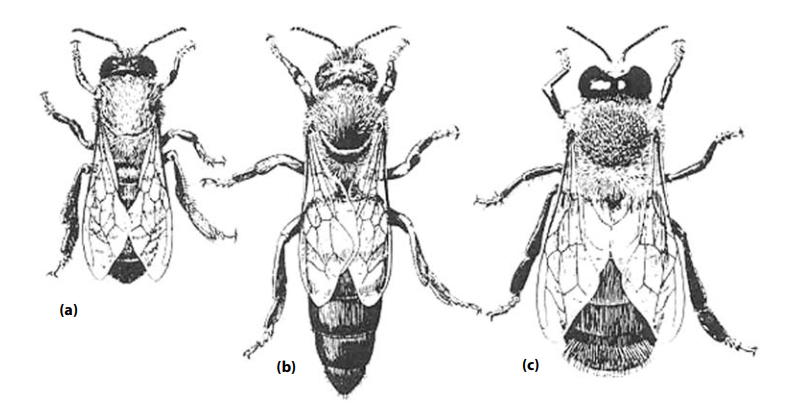
\includegraphics[width=\linewidth]{castas_de_abejas}
    \caption{Castas de abeja}
\end{figure}
\newpage
Como se observa en la figura 1, las castas son las siguientes:
\begin{enumerate}[label=\alph*)]
   \item Obreras: Estas se encargan de todas las tareas no relacionadas con la reproducción, incluyendo la construcción del panal, la recolección de polen, la producción de miel, entre otras actividades vitales para la colmena.
   \item Reinas: Son la única hembra completa de la colonia, su única responsabilidad es reproducirse y poner huevos.
    \item Drones: Similar a la reina, su única responsabilidad es reproducirse con reinas de otras colonias.
\end{enumerate}

\subsubsection{Temperatura de la colmena}
Una colmena debe de mantener una temperatura cercana a los 34 grados centígrados, para lograr esto pueden implementar ciertos mecanismos de regulación de temperatura \cite{DavidCrampABEEKEEPING}.
Cuando las abejas necesitan elevar la temperatura, generan una capa de abejas vivas alrededor de la reina, después vibran con el objetivo de producir calor. Para este proceso es necesario que la colmena cuente con suficiente alimento, además, se apoya del aislamiento de la colmena, ya sea natural o artificial, de modo natural, la miel y la cera son buenos aislantes \cite{Chadwick2016TheBook}.
Por otro lado, las abejas suelen iniciar un aleteo con sus alas para reducir la temperatura dentro de la colmena \cite{Chadwick2016TheBook}.
\subsubsection{Humedad de la colmena}
La humedad tiene un papel importante en la prevención de enfermedades dentro de la colmena, por esta razón es de importancia para las abejas controlar esta propiedad, el mecanismo que utilizan las abejas en estos casos es utilizar sus alas como ventiladores para expulsar la humedad de la colmena \cite{Chadwick2016TheBook}.
\subsubsection{Peso de la colmena}
El peso es el principal factor utilizado por los apicultores para medir la cantidad en los almacenes de miel, de manera tradicional, los apicultores intentan levantar la colmena, en caso de no ser capaces, consideran que la miel está lista para ser extraída \cite{Chadwick2016TheBook}, de manera precisa, se considera una extracción cuando el almacén de miel pesa cerca a los 40 kg \cite{DavidCrampABEEKEEPING}.
\subsubsection{Enjambrado}
El evento de enjambre sucede cuando una colonia de abejas ha sobrepasado el límite físico de la colmena en la que habita, este proceso comienza con la reina engendrando nuevas reinas y drones, después de esto un enjambre de abejas y drones emigran a un nuevo posible lugar en el cual comienza una nueva colmena \cite{Chadwick2016TheBook}.
\subsection{Internet e IoT}
El Internet de las Cosas (IoT) permite la interconexión de objetos físicos mediante tecnología y software, facilitando su monitoreo y control. Para esto, es clave una arquitectura IoT con sensores, conectividad y procesamiento de datos. Además, la inteligencia artificial puede optimizar el análisis de la información en sistemas como las colmenas inteligentes.
\subsubsection{Internet}
En el contexto actual, internet se refiere a una red global con varios protocolos de conectividad que permite comunicar paquetes de datos de dispositivos, mediante un sistema de routers, a la red \cite{RajKamal2017INTERNETPrinciples}.
\subsubsection{Rúter, router o enrutador}
Se refiere a un dispositivo capaz de almacenar direcciones y enlaces mediante las cuales se encarga de mandar paquetes de datos \cite{RajKamal2017INTERNETPrinciples}.
\subsubsection{Internet de las cosas (IOT)}
El término de internet de las coas, o IOT por sus siglas en inglés (Internet of things), se refiere al concepto de entrelazar objetos físicos dentro de una red de internet, mediante componentes electrónicos y sistemas de software, con el objetivo de permitir la comunicación entre ellos y monitorear o controlar un sistema físico \cite{RajKamal2017INTERNETPrinciples}.
\subsubsection{Arquitectura IOT}
Este concepto se refiere a la forma de estructurar u diseñar un sistema IOT y estos se dividen en capas y son 7 principales
\begin{enumerate}
   \item Componentes físicos: sensores y controladores.
   \item Dispositivos de conectividad.
   \item Computación perimetral (análisis de datos y procesamiento).
   \item Persistencia de datos.
   \item Abstracción de datos (Acceso y manipulación).
   \item Aplicación (Reportes, análisis y control).
   \item Colaboración y procesos (usuarios y procesos comerciales). 
\end{enumerate}

Estas capas sirven para estructurar y definir la arquitectura del sistema IOT \cite{RajKamal2017INTERNETPrinciples}.

\subsubsection{Sensores}
El sistema IOT interactúa con sensores, dispositivos físicos con el objetivo de adquirir datos mediante la capacidad de reaccionar a parámetros físicos como la humedad, temperatura, presión y luz y convertirla en energía eléctrica capaz de interactuar con el sistema. Durante esta interacción es posible configurar los dispositivos de manera que se ajusten a los requerimientos de la aplicación \cite{RajKamal2017INTERNETPrinciples}.
\subsubsection{Colmenas IOT}
Los términos Colmenas IOT o colmenas inteligentes se refieren a la adición de un sistema IOT a una colmena apícola, esto con el objetivo de monitorear los parámetros de la colonia de abejas y hacer accesible la información de manera que pueda ser procesada para conocer el estado de la colmena \cite{TheIAAC}.
\subsubsection{Inteligencia artificial}
Se refiere a un concepto abstracto en el cual se define a un sistema que actúa y razona de manera humana o de manera lógica \cite{Russell2022ArtificialEdition}. Es uno de los posibles métodos para procesar datos de un sistema IOT \cite{TheIAAC}.

\section{Trabajos relacionados}
\subsection{Nodos de sensores}
Este capítulo se enfoca en examinar las implementaciones de nodos de sensores. Los nodos de sensores son componentes críticos en el monitoreo de colmenas, ya que estos son los encargados de colectar datos en variables ambientales y específicas de la colmena, haciendo posible el análisis de datos y permitiendo la toma de decisiones.
\subsubsection{Embedded Software for IOT Bee Hive Monitoring Node}
Presenta un sistema embebido para monitoreo de variables relevantes, mediante un sistema que tiene las capacidades de monitorear humedad, temperatura, peso y audio. Para este sistema se utilizó el sensor SHT21 \cite{SHT21-2Sensor} para la medición de temperatura y humedad \cite{Vidrascu2017EmbeddedNode}.
\subsubsection{A Smart Sensor-Based Measurement System for Advanced Bee Hive Monitoring}
Desarrolla un sistema de monitoreo de parámetros relevantes para la colmena, incluyendo peso, sonido, temperatura, humedad y CO2. El objetivo es desarrollar un sistema que de una visión general del ambiente interno y externo de la colmena.
Este sistema es modular y se compone de dos módulos principales:
\begin{itemize}
    \item Módulo Abeja: Este módulo se instala en cada colmena y está constituido por un módulo Raspberry pi 3B \cite{BuyPi}, una tarjeta de sonido UCA22 \cite{BehringerUCA222}, dos micrófonos ADMP401 MEMS \cite{ADMP401Devices} dos sensores de humedad y temperatura DHT22 \cite{LiuDigital-outputModule/sensor}, células de carga TAL220 \cite{LoadElectronics} con el módulo interfaz HX711\cite{HX711Electronics} y un sensor de CO2 TL6615 \cite{T6615Telaire}.
    \item Módulo Reina: Este módulo se instala cerca del grupo de modulos abeja y se encarga de recolectar la información de los mismos. También está constituido por una Raspberry pi 3B y un puente 5 g (no especificado) utilizado para comunicarse con el servidor remoto \cite{Cecchi2020AMonitoring}.
\end{itemize}
El sistema de micrófonos recopila muestras de 30 segundos cada 10 minutos, a una tasa de 32 kHz

\subsubsection{High Reliability Wireless Sensor Node for Bee Hive Monitoring}
Propone un sistema diseñado para condiciones ambientales de entre -20 a 60 grados centígrados y con una arquitectura principalmente modular, permitiendo intercambiar sensores según se requiera, esto mediante la interfaz digital I2C \cite{Vidrascu2016HighMonitoring}.
Se denota la importancia de utilizar sensores de temperatura y humedad, principalmente durante el invierno, para prevenir la formación de rocío dentro de la colmena. El sensor de temperatura utilizado fue un SHT21 de Sensirion, este sensor tiene un consumo de 1 mW en modo medición y 1 micro Watts en modo inactivo \cite{Vidrascu2016HighMonitoring}.
Se utiliza el sistema de medición de peso HX711 de Avia Semiconductor que consta de un sistema de alimentación, un amplificador y un convertidor analógico digital de 24-bit, en conjunto con 4 células de carga. Todo este sistema tiene un consumo de 8.25 mW en modo activo y 5.5 µW en modo inactivo \cite{Vidrascu2016HighMonitoring}.
Adicionalmente, el sistema cuenta con un sensor de inclinación DMA08 para monitorear si la colmena está nivelada, si ha sido robada y detectar caídas \cite{Vidrascu2016HighMonitoring}.
El sistema también cuenta con un micrófono MP34DT05-A, la justificación para este el elemento es que es útil para detectar eventos de enjambre y escasez de comida en el invierno \cite{Vidrascu2016HighMonitoring}.

\subsubsection{Bee Swarm Activity Acoustic Classification for an IoT-Based Farm Service}
En esta investigación se procesa información recopilada de un sistema que utiliza un micrófono TDK InvenSense ICS-40300 y una placa Atmel ATmega32U4 sobre la colmena para posteriormente ser procesada en un servidor remoto \cite{Zgank2019BeeService}.
\subsubsection{Maintenance-free IOT Gateway Design for Bee Hive Monitoring}
El módulo descrito en este artículo tiene las capacidades de recopilar información importante sobre el estado de la colmena mediante: un sensor SHT21 para medir humedad y temperatura, un sensor de presión atmosférica MPL3115A2 \cite{NXPBVMPL3115A2Sheet}, un sensor de intensidad lumínica TSL2561 \cite{OverviewSystem}, células de carga HX711 colocadas con el objetivo de monitorear el peso de la colmena, un sensor de radiación UV VEML6075 \cite{AdafruitKits} y finalmente, un sensor de concentración de polvo GP2Y1010AU0F \cite{SensorGP2Y1010AU0F} \cite{Vidrascu2017Maintenance-freeMonitoring}.
\subsubsection{A Pi-Based IoT System Design}
En este Sistema se integra la suite de sensores de GrovePi \cite{GrovePiKit}, en concreto los sensores de humedad, temperatura, GPS, sonido e imágenes térmicas \cite{Chen2020ADesign}.
\subsection{Sistema de transmisión de datos}
Este capítulo se centra en los sistemas de transmisión de datos utilizados en estos sistemas, presentando diversas soluciones de hardware y software que permiten la transmisión eficiente de datos desde las colmenas hasta las plataformas de análisis y monitoreo remoto.
\subsubsection{Embedded Software for IOT Bee Hive Monitoring Node}
El sistema está construido alrededor del componente ESP8266 que integra un microcontrolador Tensilica L106 32-bit en conjunto con el módulo transmisor wifi que integra circuitos de radiofrecuencia y es capaz de transmitir datos mediante interfaces digitales como SPI, I2C, y UART. Además, el módulo ESP8266 cuenta con tres modos de operación: activo, dormido y dormido profundo, los cuales son aprovechados por el sistema para optimizar el uso de energía \cite{Vidrascu2017EmbeddedNode}.
\subsubsection{High Reliability Wireless Sensor Node for Bee Hive Monitoring}
En este sistema también se utiliza un módulo ESP8266 serie 32-bit a 80 MHz, el objetivo de utilizar este componente es simplificar el diseño utilizando la capacidad del componente para una conexión wifi directa \cite{Vidrascu2016HighMonitoring}.
\subsubsection{Maintenance-free IOT Gateway Design for Bee Hive Monitoring}
El módulo ESP8266 es de nuevo utilizado en este sistema, en concreto la versión ESP8266-12\cite{ModuloESP-12E} producido por A.I. Thinker para dar conectividad al módulo que contiene el nodo de sensores. Adicionalmente, en este proyecto se agrega un modem A6 GSM/GPRS \cite{THIDOA6} que sirve como compuerta para conectar los módulos a la red 5G \cite{Vidrascu2017Maintenance-freeMonitoring}.
\subsubsection{A Pi-Based IoT System Design}
Este sistema también implementa el método de múltiples módulos con conexión WIFI conectados a un modem independiente que se conecta a la red móvil para proveer de internet a los módulos \cite{Chen2020ADesign}.
\subsection{Manejo de energía}
Este capítulo examina las diversas estrategias de manejo de energía implementadas en sistemas de monitoreo avanzado de colmenas. Desde la conexión a la red eléctrica hasta soluciones autónomas con energía solar y súper capacitores. 
\subsubsection{A Smart Sensor-Based Measurement System for Advanced Bee Hive Monitoring }
En este artículo se energiza mediante una conexión a la red eléctrica, los módulos Reina y Abeja consumen 4 y 4.2 watts respectivamente \cite{Cecchi2020AMonitoring}.
\subsubsection{Maintenance-free IOT Gateway Design for Bee Hive Monitoring}
En esta investigación, la energía se obtiene utilizando paneles solares (no especificado) en conjunto con un módulo LT3652\cite{LT3652Devices} que regula la cantidad de voltaje de salida del panel solar para maximizar la transferencia de energía. Además, se utiliza un cargador LTC3652\cite{LTC3652Technology} para ajustar el voltaje de carga de los súper capacitores al voltaje especificado por el módulo LT3652 \cite{Vidrascu2017Maintenance-freeMonitoring}.
\subsubsection{A Pi-Based IoT System Design}
En este sistema se cuenta con una batería para dispositivos celulares con una capacidad de 10000 mAh (180000 Joules a 5 V) que mantiene el sistema encendido entre 27 y 33 horas \cite{Chen2020ADesign}.
\subsection{Procesamiento de datos}
El capítulo se enfoca en el procesamiento de datos acústicos para la detección de eventos de enjambre en un servicio agrícola basado en IoT.
\subsubsection{Bee Swarm Activity Acoustic Classification for an IoT-Based Farm Service}
Como ya se mencionó, el enfoque de esta investigación es el procesamiento de datos acústicos con el objetivo de detectar eventos de enjambre, el recurso principal para el desarrollo del modelo es el proyecto de fuente abierta de colmenas Open Source Beehives Project (OSBP).
Los datos de entrenamiento fueron recopilados del OSBP, los cuales consistieron de alrededor de 122 minutos de audio a los cuales se les disminuyo la frecuencia a 16 kHz, la resolución a 16 bits y fueron divididos en muestras de 3 segundos, resultando en 1800 muestras destinadas para entrenamiento y 643 para pruebas. Se tomó la precaución de utilizar muestras de una sola colmena.
El diseño experimental se desarrolló utilizando referencias de reconocimiento del habla, de este modo, se desarrollaron dos procesos, los cuales consistieron en aplicar una extracción de características al audio para generar un vector de características que posteriormente sería clasificado.
Para la extracción de características se utilizaron 2 métodos:
\begin{itemize}
\item Mel-Frequency Cepstral Coefficients (MFCC): Este es el principal método para la extracción de características, el resultado de este proceso fue un vector con 12 coeficientes Mel-Frequency Cepstral a los cuales se les sumó un coeficiente de energía. Posteriormente, se calcularon y añadieron las derivadas de primero y segundo orden para los primeros 13 elementos, lo que resulto en 39 coeficientes.
\item Linear Predictive Coding (LFC): Este método fue secundario y utilizado como comparación, durante este proceso también se aplicó una sustracción espectral para reducir el ruido de fondo. Este método requiere una señal en el dominio de la frecuencia, por lo que se utilizó una transformada rápida de Fourier (Fast Fourier Transform, FFT) para transformar la frecuencia.
\end{itemize}

En cuanto a la clasificación de muestras se utilizaron 2 métodos paralelos:
\begin{itemize}
\item Hidden Markov Model (HMM): Este método se desarrolló con 2 topologías, una con 15 estados, similar a los modelos de reconocimiento del habla, y otra con 1 estado, similar a los modelos de GMM.
\item Gaussian Mixture Model (GMM): Para este modelo se inició con la inicialización plana de parámetros y se continuó con la re-estimación de Baum-Welch, repitiendo el proceso hasta alcanzar 32 mezclas de PDF Gaussianas por estado \cite{TheIAAC} \cite{Zgank2019BeeService}.
\end{itemize}

\section{Arquitectura del sistema}

\begin{figure}[h]
    \centering
    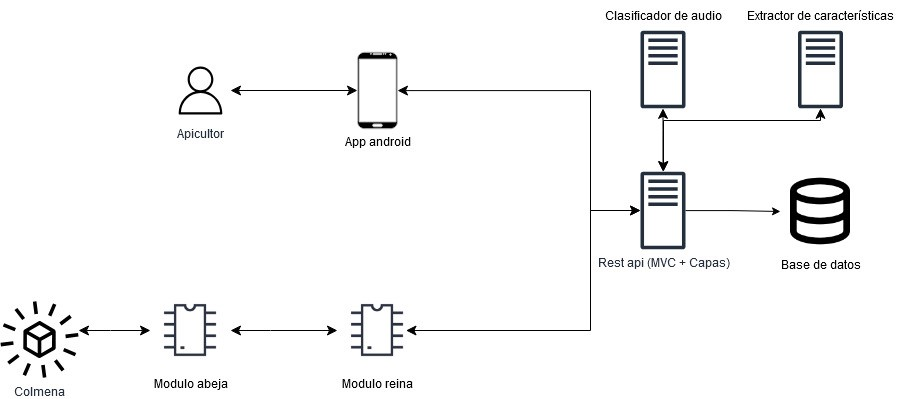
\includegraphics[width=\linewidth]{arquitectura_sistema}
    \caption{Arquitectura general del sistema}
\end{figure}

\begin{figure}[h]
    \centering
    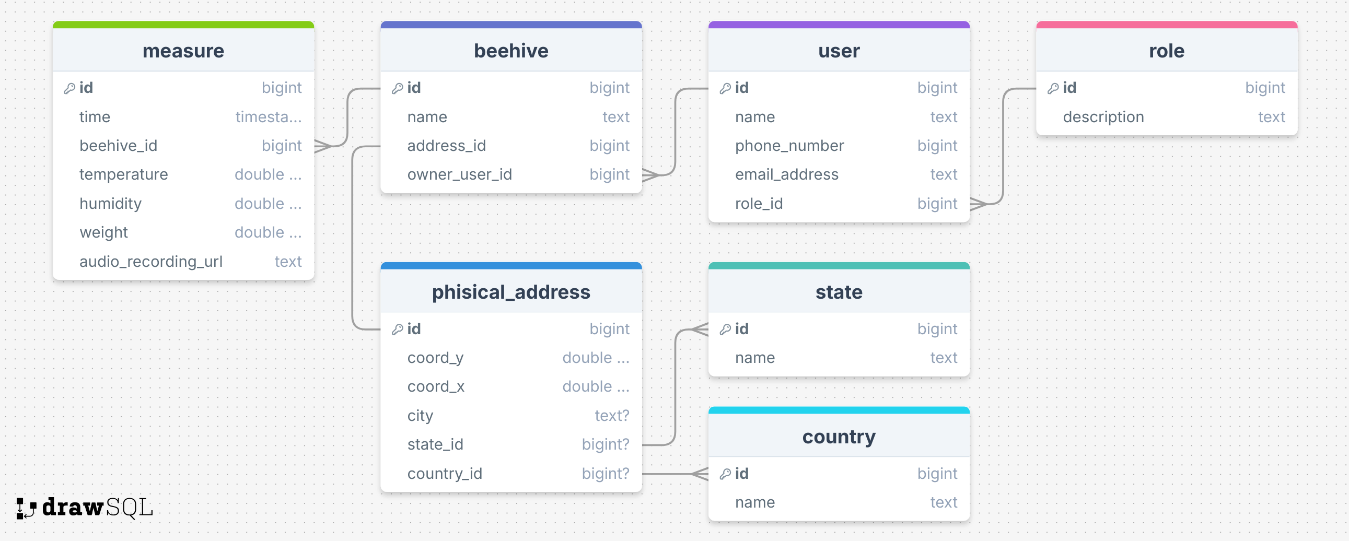
\includegraphics[width=\linewidth]{diagrama_er}
    \caption{Diagrama de la base de datos}
\end{figure}

\section{Conclusiones}

El diseño e implementación de un sistema inteligente basado en IoT para el monitoreo de colmenas apícolas permite mejorar la eficiencia y efectividad del monitoreo de las colmenas. La integración de sensores para medir parámetros como temperatura, humedad, peso y audio, junto con el reconocimiento de patrones, tiene potencial para facilitar la detección temprana de problemas y la toma de decisiones informadas.

\printbibliography[title={REFERENCIAS}]

\end{document}